% Set the document class and theme
\documentclass{beamer}
\usetheme{CambridgeUS}
\setbeamertemplate{caption}[numbered]
\setbeamertemplate{theorems}[numbered]

\usepackage{./presentation_macros}

% Add presentation data here

% Text in the square brackets `[]' are shown in the footer. If not mentioned,
% then text in the curly braces `{}' are used as theme defaults.

\title[QUIC-FL]{QUIC-FL: Quick UnbIased Compression for Federated Learning\\
\small Ran Ben Basat, Shay Vargaftik, Amit Portnoy, Gil Einziger, Yaniv Ben-Itzhak, Michael Mitzenmacher}
\date{November 22, 2023}
\author{Gautam Singh}
\institute[]{Indian Institute of Technology Hyderabad}

% Presentation begins here

\begin{document}
    \maketitle
    \tableofcontents
    \section{Introduction}

    \begin{frame}
        \frametitle{The DME Problem}
        \begin{figure}[!ht]
            \begin{tikzpicture}[node distance = 5ex]
    \node[state] (C_1) {$C_1$}; 
    \node[state] (C_2) [right=of C_1] {$C_2$}; 
    \node (L) [right=of C_2] {$\ldots$};
    \node[state] (C_n) [right=of L] {$C_n$}; 
    \node[state,rectangle] (S) [above=of $(C_2.north)!0.5!(L.north)$] {$S$};
    \node (X_1) [below=of C_1] {$\vect{X_1} \in \bR^d$};
    \node (X_2) [below=of C_2] {$\vect{X_2}$};
    \node (X_n) [below=of C_n] {$\vect{X_n}$};
    \node (L1) [below=of L] {$\ldots$};
    \node (muhat) [above=of S] {$\hat{\vect{\mu}} \triangleq \frac{1}{n}\sum_{i=1}^n\hat{\vect{X_i}}$}; 
    \path[->]
    (C_1) edge  node [left=1ex] {$\vect{Y_1} \in \cbrak{0,1}^b$} (S)
    (C_2) edge  node [right=1ex] {$\vect{Y_2}$} (S)
    (C_n) edge  node [right=1ex] {$\vect{Y_n}$} (S)
    (S) edge node {} (muhat)
    (X_1) edge node {} (C_1)
    (X_2) edge node {} (C_2)
    (X_n) edge node {} (C_n);
\end{tikzpicture}
            \caption{Illustration of the DME Problem. Here, \(\hat{\vect{X_i}}\)
            denotes the server estimate for \(\vect{X_i}\).} 
            \label{fig:dme}
        \end{figure}
    \end{frame}

    \section{Preliminaries}
    \begin{frame}
        \frametitle{vNMSE and NMSE}
        \begin{definition}[vNMSE]
        The \emph{vector Normalized Mean Square Error} of \(\vect{x}\)
        is defined as
        \begin{equation}
            vNMSE \triangleq \frac{\mean{\norm{\hat{\vec{x}}-\vec{x}}^2_2}}{\norm{\vect{x}}^2_2}.
            \label{eq:vnmse-def}
        \end{equation}
        \end{definition}
        \begin{definition}[NMSE]
        The \emph{Normalized Mean Square Error} in the case of the DME
        problem is defined as
        \begin{equation}
            NMSE \triangleq \frac{\mean{\norm{\hat{\vect{\mu}}-\vect{\mu}}^2_2}}{\frac{1}{n}\sum_{i=1}^n\norm{\vect{x}_i}^2_2} = \frac{\mean{\norm{\hat{\vect{\mu}}-\frac{1}{n}\sum_{i=1}^n\vect{x}_i}^2_2}}{\frac{1}{n}\sum_{i=1}^n\norm{\vect{x}_i}^2_2}.
            \label{eq:nmse-def}
        \end{equation}
        \end{definition}
    \end{frame}

    \begin{frame}
        \frametitle{An Important Lemma}
        \begin{lemma}
            \label{lem:vnmse-nmse-rel}
            For \(n\) clients with unbiased and independent estimates, we have
            \cite{EDEN}
            \begin{equation}
                NMSE = \frac{\sum_{i=1}^nvNMSE\brak{i}\norm{\vect{x}_i}_2^2}{n\sum_{i=1}^n\norm{\vect{x}_i}_2^2}
                \label{eq:vnmse-nmse-rel}
            \end{equation}
        \end{lemma}
        \begin{corollary}
            \label{cor:vnmse-nmse-ball}
            If all clients have the same \(vNMSE\), then
            \begin{equation}
                NMSE = \frac{vNMSE}{n}
                \label{eq:vnmse-nmse-ball}
            \end{equation}
        \end{corollary}
        From the above lemma, we need the \(vNMSE\) to be a constant so that the
        \(NMSE\) is \(\cO\brak{1/n}\) for QUIC-FL.
    \end{frame}

    \begin{frame}
        \frametitle{Randomized Hadamard Transform}
        \begin{definition}[Walsh-Hadamard Matrix]
            The Walsh-Hadamard matrix \(\vect{H}_{2^k}\) with \(\vect{H}_1 = 
            \myvec{1}\) is recursively defined as
            \begin{equation}
                \vect{H}_{2^k} = \myvec{\vect{H}_{2^{k-1}} & \vect{H}_{2^{k-1}} \\ \vect{H}_{2^{k-1}} & -\vect{H}_{2^{k-1}}}.
                \label{eq:Hl-def}
            \end{equation}
        \end{definition}
        \begin{definition}[Randomized Hadamard Transform]
            Let \(\vect{H}\in\cbrak{-1,+1}^{d\times d}\) be a Walsh-Hadamard 
            Matrix and \(\vect{D}\) be a diagonal matrix with uniform iid 
            Rademacher entries \emph{i.e.}, entries that are \(\pm 1\) with 
            equal probability. Then, the \emph{randomized Hadamard transform} 
            (RHT) of \(\vect{x}\in\bR^d\) is given by
            \begin{equation}
                \cR_{\vect{H}}\brak{\vect{x}} \triangleq \brak{\frac{1}{\sqrt{d}}\vect{HD}}\vect{x}.
                \label{eq:rht-def}
            \end{equation}
        \end{definition}
    \end{frame}

    \begin{frame}
        \frametitle{Properties of RHT}
        \begin{definition}[Inverse RHT]
            The \emph{inverse randomized Hadamard transform} of \(\vect{x}\) is given by
            \begin{equation}
                \cR_{\vect{H}}^{-1}\brak{\vect{x}} \triangleq \brak{\frac{1}{\sqrt{d}}\vect{DH}}\vect{x}.
                \label{eq:inv-rht-def}
            \end{equation}
        \end{definition}
        \begin{lemma}
            \label{lem:rht-norm-conv}
            Define \(F_{i,d}\brak{x}\) to be the CDF of
            \(\frac{1}{\sigma}\cR_{\vect{H}}\brak{\vect{x}}_i\), where
            \(\mean{x_i^2} = \sigma^2\), and \(\Phi\brak{x}\) the CDF of the
            standard normal distribution. Then, as \(d\to\infty\), \(\forall\ 1
            \le j \le d\), 
            \begin{equation}
                F_{i,d}\brak{x_j} \xrightarrow{\mathrm{d}} \Phi\brak{x_j}.
                \label{eq:rht-norm-conv}
            \end{equation}
        \end{lemma}
    \end{frame}

    \begin{frame}
        \frametitle{Design Goals of QUIC-FL}
        \begin{enumerate}
            \item Less computational complexity compared to other methods, at
            \emph{both} client and server.
            \item Same (asymptotic) NMSE as other methods: \(\cO\brak{\frac{1}{n}}\).
            \item Better compression ratio.
        \end{enumerate}
    \end{frame}

    \section{Bounded Support Quantization (BSQ)}
    \begin{frame}
        \frametitle{BSQ Algorithm}
        \begin{enumerate}
            \item Uses a parameter \(p\in\rsbrak{\lbrak{0,1}}\), based on which 
            a threshold  \(\sbrak{-t_p,t_p}\) is chosen such that at most \(dp\)
            values lie outside this interval.
            \item \(\vect{x}\) separated into two parts: \emph{large}
            values that lie outside this interval and \emph{small} values
            that lie inside this interval.
            \item To encode \(\vect{x}\),
            \begin{enumerate}
                \item \emph{Large} values are sent exactly, along with their
                indices. Costs \(\log\binom{d}{dp} \approx 
                dp\log\brak{\frac{1}{p}}\) bits. Can use delta encoding or
                no encoding at cost of \(dp\ceil{\log d}\) bits (Authors assume
                \(p\log d << 1\)).
                \item \emph{Small} values are stochastically quantized and sent
                using \(b\) bits per coordinate. \emph{This implies that BSQ is
                unbiased}.
            \end{enumerate}
            \item To decode and compute \(\hat{\vect{x}}\), decode the
            \emph{large} values along with their indices. Then, estimate the
            quantized \emph{small} values.
        \end{enumerate}
    \end{frame}

    \begin{frame}
        \frametitle{Main Result of BSQ}
        \begin{lemma}
            BSQ, without further assumptions, admits a worst-case NMSE of
            \(\frac{1}{np\brak{2^b-1}^2}\) with \(\cO\brak{d}\) and
            \(\cO\brak{nd}\) complexity for encoding and decoding respectively.
        \end{lemma}
        \begin{exampleblock}{Arbitrarily Large NMSE}
            Notice that the constant in the NMSE can be made arbitrarily large.
            For example, \(p = 2^{-10},\ b = 1\).
        \end{exampleblock}
        \begin{alertblock}{What QUIC-FL Does}
            The \textbf{random rotation preprocessing} applied by QUIC-FL
            guarantees smaller constant values for small \(p\).
        \end{alertblock}
    \end{frame}
    
    \section{Distribution-Aware Unbiased Quantization}
    \begin{frame}
        \frametitle{Distribution-Aware Unbiased Quantization\\\small Key Idea}
        We have \(\forall\ 1 \le i \le d\), where \(\vect{R}\) denotes a random
        rotation matrix \cite{vargaftik2021drive},
        \begin{equation}
            \frac{\sqrt{d}}{\norm{\vect{x}}_2}\brak{\vect{Rx}}_i \sim \cN\brak{0,1}.
            \label{eq:rot-norm-conv}
        \end{equation}
        Thus, we only need to optimize the reconstruction values for when the
        data is sampled from the \emph{standard normal distribution}. This will
        yield a \emph{near-optimal} quantization for the \(\vect{x}_i\).

        Notice that this is possible since
        \begin{enumerate}
            \item We know the distribution of the transformed vector by
            \eqref{eq:rot-norm-conv}.
            \item We know the range \(\sbrak{-t_p, t_p}\) of \(\vect{x}_i\).
        \end{enumerate}
    \end{frame}
    
    \begin{frame}
        \frametitle{Distribution-Aware Unbiased Quantization\\\small Definitions}
        \begin{table}[!ht]
            \centering
            \begin{tabular}{|c|c|}
                \hline
                \textbf{Notation} & \textbf{Definition} \\
                \hline
                \(p\) & BSQ parameter \\
                \hline
                \(t_p\) & BSQ threshold \\
                \hline
                \(b\) & Number of bits per quantized value \\
                \hline
                \(\cM\) & Message space \(\cbrak{0,1,\ldots,2^b-1}\) \\
                \hline
                \(R\brak{x}\) & Reconstruction point associated with \(x\) at the receiver \\
                \hline
                \(\cQ_{b,p}\) & Set of all reconstruction points \(\cbrak{R\brak{x}\ |\ x \in \cM}\) \\
                \hline
                \(\cI_m\) & \(\cbrak{0,1,\ldots,m-1}\) \\
                \hline
                \(\cA_{p,m}\brak{i}\) & \(\pr{Z \le \cA_{p,m}\brak{i}\ |\ Z \in \sbrak{-t_p,t_p},\ Z \sim \cN\brak{0,1}} = \frac{i}{m-1}\) \\
                \hline
                \(\cA_{p,m}\) & Right endpoints of quantiles \(\cbrak{\cA_{p,m}\brak{i}\ |\ i\in\cI_m}\) \\
                \hline
                \(S\brak{z,x}\) & \(\pr{z \text{ is quantized to } R\brak{x}}\) \\
                \hline
                \(S^\prime\brak{i,x}\) & \(S\brak{\cA_{p,m}\brak{i}, x}\) \\
                \hline
            \end{tabular}
            \caption{Notation for Distribution-Aware Unbiased Quantization.}
            \label{tab:dauq-defs}
        \end{table}
    \end{frame}

    \begin{frame}
        \frametitle{Distribution-Aware Unbiased Quantization\\\small Optimization Problem}
        We want to minimize the MSE of this scheme. The optimization problem
        becomes

        \begin{align}
            \min_{S,R} \int_{-t_p}^{t_p} &\sum_{x\in\cM}S\brak{z,x}\brak{z-R\brak{x}}^2e^{-\frac{z^2}{2}}dz\ \text{s.t.} \\
            \text{(Probability)} &\sum_{x\in\cM}S\brak{z,x} = 1 \\
            \text{(Unbiasedness)} &\sum_{x\in\cM}S\brak{z,x}R\brak{x} = z.
            \label{eq:opt-prob-dauq}
        \end{align}

        \emph{This is not easy to solve!}
    \end{frame}

    \begin{frame}
        \frametitle{Distribution-Aware Unbiased Quantization\\\small Discretization}
        Can now use solvers like APOPT \cite{APOPT} and IPOPT \cite{IPOPT} to
        solve for \(\cQ_{b,p}\). 

        \begin{align}
            \min_{\red{S^\prime},R} &\sum_{\substack{\red{i\in\cI_m}\\x\in\cM}}\red{S^\prime}\brak{\red{i},x}\brak{\red{\cA_{p,m}\brak{i}}-R\brak{x}}^2 \text{ s.t.} \\
            \text{(Probability)} &\sum_{x\in\cM}\red{S^\prime}\brak{\red{i},x} = 1 \\
            \text{(Unbiasedness)} &\sum_{x\in\cM}\red{S^\prime}\brak{\red{i},x}R\brak{x} = \red{\cA_{p,m}\brak{i}}.
            \label{eq:opt-prob-dauq-disc}
        \end{align}

        The reconstruction points \(\cQ_{b,p}\) obtained correspond to a
        \emph{near-optimal} solution.
        \begin{enumerate}
            \item Convergence of randomly rotated coordinates to normal
            distribution, from \eqref{eq:rot-norm-conv}.
            \item As \(m\to\infty\), the discrete problem converges to the
            continuous version.
        \end{enumerate}
    \end{frame}

    \section{The QUIC-FL Algorithm}

    \begin{frame}
        \frametitle{QUIC-FL Client}
        \begin{algorithm}[H]
            \caption{QUIC-FL Client}
            \label{alg:quic-fl-client}
            \begin{algorithmic}[1]
                \Require{BSQ parameter \(p\) and threshold \(t_p\), bits per
                symbol \(b\), global randomness \(T\), precomputed
                reconstruction values \(\cQ_{b,p}\), stochastic quantization
                algorithm \(Q\).}
                \Procedure{QUICFLClient}{$\vect{x}_c$}
                \State $\vect{Z}_c \gets \frac{\sqrt{d}}{\norm{\vect{x}_c}_2}T\brak{\vect{x}_c}$
                \State $\vect{U}_c \gets \cbrak{Z_{ci}\ |\ \abs{Z_{ci}} > t_p}$
                \State $\vect{I}_c \gets \cbrak{i\ |\ \abs{Z_{ci}} > t_p}$
                \State $\vect{V}_c \gets \cbrak{Z_{ci}\ |\ \abs{Z_{ci}} \le t_p}$
                \State $\vect{X}_c \gets Q\brak{\vect{V}_c}$ using $\cQ_{b,p}$
                \State Send $\brak{\norm{\vect{x}_c}_2, \vect{U}_c, \vect{I}_c, \vect{X}_c}$ to server
                \EndProcedure
            \end{algorithmic}
        \end{algorithm}
    \end{frame}

    \begin{frame}
        \frametitle{QUIC-FL Server}
        \begin{algorithm}[H]
            \caption{QUIC-FL Server}
            \label{alg:quic-fl-server}
            \begin{algorithmic}[1]
                \Require{BSQ parameter \(p\) and threshold \(t_p\), bits per
                symbol \(b\), global randomness \(T\), precomputed
                reconstruction values \(\cQ_{b,p}\), stochastic quantization
                algorithm \(Q\), subrountine \textsc{Merge} to reconstruct
                quantized vector given its BSQ parts.}
                \Procedure{QUICFLServer}{}
                \ForAll{$1 \le c \le n$}
                    \State $\hat{\vect{V}}_c \gets \cbrak{\cQ_{b,p}\brak{x} \text{ for } x \text{ in } \vect{X}_c}$
                    \State $\hat{\vect{Z}}_c \gets \textsc{Merge}\brak{\hat{\vect{V}}_c, \vect{U}_c, \vect{I}_c}$
                \EndFor
                \State $\hat{\vect{\mu}}_Z \gets \frac{1}{n}\sum_{c=1}^{n}\frac{\norm{\vect{x}_c}_2}{\sqrt{d}}\hat{\vect{Z}}_c$
                \State $\hat{\vect{\mu}} \gets T^{-1}\brak{\hat{\vect{\mu}}_Z}$
                \EndProcedure
            \end{algorithmic}
        \end{algorithm}
    \end{frame}

    \begin{frame}
        \frametitle{NMSE of QUIC-FL}    
        \begin{theorem}
            Let \(Z\sim\cN\brak{0,1}\) and \(\hat{Z}\) be its estimate using the
            distribution-aware unbiased quantization scheme. Then, for any
            number of clients \(n\) and any set of input vectors
            \(\cbrak{\vec{x}_i \in\bR^d\ |\ i\in\cbrak{0,1,\ldots,n-1}}\), the
            NMSE of QUIC-FL is given by
            \begin{equation}
                NMSE = \frac{1}{n}\mean{\brak{Z-\hat{Z}}^2} + \cO\brak{\frac{1}{n}\sqrt{\frac{\log d}{d}}}
                \label{eq:quic-fl-nmse}
            \end{equation}
        \end{theorem}

        When \(d\to\infty\), the NMSE respects \(\cO\brak{\frac{1}{n}}\).
    \end{frame}

    \begin{frame}
        \frametitle{Optimizations\\\small Client-Specific Shared Randomness}
        Some amount of random bits are shared between each client and the
        server. This can reduce the MSE at the cost of generating more random
        bits.

        Define the following quantities.

        \begin{enumerate}
            \item \(l\), the number of random bits used.
            \item \(\cH_l \triangleq \cbrak{0,1,\ldots,2^l-1}\), the set of all
            possible random bitstrings of length \(l\).
            \item \(H \sim \cU\sbrak{\cH_l}\), the random variable representing
            the shared randomness, selected uniformly from \(\cH_l\).
            \item \(S^\prime\brak{h,i,x} \triangleq \pr{\cA_{p,m}\brak{i} \text{
            is quantized to } R\brak{H, x}\ |\ H = h}\).
            \item \(R\brak{h,x}\), the reconstruction point for \(x\in\cM\)
            given shared randomness \(h\).
        \end{enumerate}
    \end{frame}

    \begin{frame}
        \frametitle{Optimizations\\\small Client-Specific Shared Randomness}
        The new optimization problem becomes the following.
        \begin{align}
            \min_{S^\prime,R} &\sum_{\substack{\red{h\in\cH_l}\\i\in\cI_m\\x\in\cM}}S^\prime\brak{\red{h},i,x}\brak{\cA_{p,m}\brak{i} - R\brak{\red{h},x}}^2 \text{ s.t.} \\
            \text{(Probability)} &\sum_{x\in\cM}S^\prime\brak{\red{h},i,x} = 1 \\
            \text{(Unbiasedness)} &\red{\frac{1}{2^l}}\sum_{\substack{\red{h\in\cH_l}\\x\in\cM}}S^\prime\brak{\red{h},i,x}R\brak{\red{h},x} = \cA_{p,m}\brak{i}.
            \label{eq:opt-quic-fl-rand}
        \end{align}
    \end{frame}

    \begin{frame}
        \frametitle{Optimizations\\\small Using the RHT}    
        \begin{enumerate}
            \item Accelerates both client and server algorithms.
            \item Same asymptotic guarantees but with larger constants. 
            \begin{enumerate}
                \item For the RHT, \(\mean{\brak{Z-\hat{Z}}^2} = \cO\brak{p}\).
                \item Can compensate by slight increase in \(b\).
                \item The guarantees on the constant are still better than DRIVE
                and EDEN.
            \end{enumerate}
            \item Fastest complexity in comparison to other state-of-the-art
            methods, at both client and server.
        \end{enumerate}
    \end{frame}
    
    \section{Results}
    \begin{frame}
        \frametitle{Complexity Analysis}
        \begin{table}
            \centering
            \begin{tabular}{|c|c|c|c|}
                \hline
                \textbf{Algorithm} & \textbf{Enc. Complexity} & \textbf{Dec. Complexity} & \textbf{NMSE} \\
                \hline 
                \textbf{QSGD} & \(\cO\brak{d}\) & \(\cO\brak{nd}\) & \(\cO\brak{d/n}\) \\
                \hline
                \textbf{Hadamard} & \(\cO\brak{d\log d}\) & \(\cO\brak{nd + d\log d}\) & \(\cO\brak{\log d/n}\) \\
                \hline
                \textbf{Kashin} & \(\cO\brak{d\log d\log\brak{nd}}\) & \(\cO\brak{nd + d\log d}\) & \(\cO\brak{1/n}\) \\
                \hline
                \textbf{EDEN} & \(\cO\brak{d\log d}\) & \(\cO\brak{nd\log d}\) & \(\cO\brak{1/n}\) \\
                \hline
                \textbf{QUIC-FL} & \(\cO\brak{d\log d}\) & \(\cO\brak{nd + d\log d}\) & \(\cO\brak{1/n}\) \\
                \hline
            \end{tabular}
            \caption{Complexities and NMSE of Unbiased DME Algorithms.}
            \label{fig:quic-fl-comp}
        \end{table}
    \end{frame}

    \begin{frame}
        \frametitle{Accuracy}    
        \begin{figure}
            \centering
            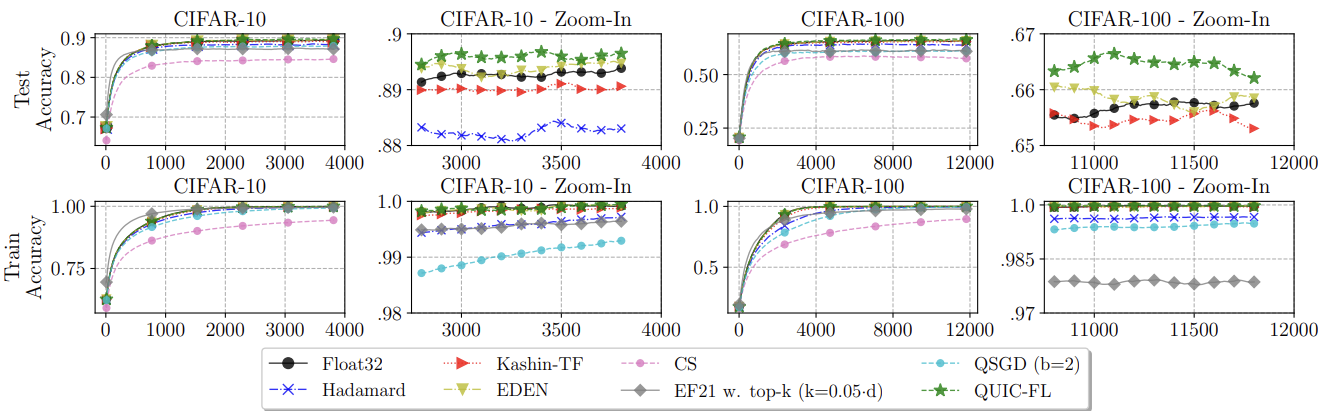
\includegraphics[width=\columnwidth]{images/results.png}
            \caption{Cross-device Federated Learning with Various Methods of
            Unbiased Quantization. \cite{basat2023quicfl}}
            \label{fig:quic-fl-acc}
        \end{figure}
    \end{frame}

    \section{Further Improvements}
    \begin{frame}
        \frametitle{Further Improvements in QUIC-FL}    
        \begin{enumerate}
            \item (Open problem) Using more than one RHT can lead to better
            bounds?
            \item QUIC-FL for cases using limited bits \(b\) and dimensions
            \(d\).
            \item Space complexity per client? Better compression ratio?
            \begin{enumerate}
                \item Depends on \(d\), \(b\) and \(p\).
            \end{enumerate}
            \item Can the NMSE be lowered using a client-server feedback system?
            \item Security concerns
            \begin{enumerate}
                \item Does the random transformation \(T\) act as a ``secret
                key''?
                \item What security guarantees does QUIC-FL have against various
                adversarial attacks?
            \end{enumerate}
        \end{enumerate}
    \end{frame}

    \section{References}
    \begin{frame}[allowframebreaks]
        % \frametitle{References}
        \bibliography{references.bib}
    \end{frame}
\end{document}
